\section{Probabilistic deformation model}
\label{sec:part_representation_learning}

Our method takes as input a collection of shapes, and outputs groups of structurally similar shapes together with learned \rev{part templates} per group (Figure \ref{fig:hierarchy}). Given the group-specific \rev{part templates}, our method also outputs high-level \rev{part templates} for the whole collection. A probabilistic model is used to infer the \rev{part templates}. The model evaluates the joint probability of hypothesized \rev{part templates}, deformations of these \rev{templates} towards the input shapes, as well as shape correspondences and segmentations. The probabilistic model is defined over the following set of random variables:
\begin{description}[leftmargin=1em]
\setlength{\itemsep}{4pt}
\setlength{\parskip}{0pt}
\setlength{\parsep}{0pt}
\item[Part templates] $\bY = \{\bY_k\}$ where $\bY_k \in  \mathbb{R}^3$ denotes the 3D position of a point $k$ on a latent \rev{part template}. There are total $K$ such variables, where $K$ is the  number of points on all \rev{part templates}. The number of points per \rev{part template} is determined from the provided exemplar shape parts. 
\item[Deformations] $\bD = \{\bD_{t,k}\}$ where $\bD_{t,k} \in \mathbb{R}^3$ represents the position of a point $k$ on a \rev{part template} as it deforms towards the shape $t$. Given $T$ input shapes and $K$ total points across all \rev{part templates}, there are  $K \cdot T$ such variables. 
\item[Point correspondences] $\bU = \{U_{t,p}\}$ where $U_{t,p} \in \{1,2,...,K\}$ represents the ``fuzzy'' correspondence of the surface point $p$ on an input shape $t$ with points on the \rev{part templates}. In our implementation, each input shape is uniformly sampled with $5000$ points, thus there are total  $5000 \cdot T$ such random variables. 
\item[Surface segmentation] $\bS = \{S_{t,p}\}$ where $S_{t,p} \in \{1,...,L\}$ represents the part label for a surface point $p$ on an input shape $t$. $L$ is the number of available \rev{part templates}, corresponding to the total number of semantic part labels. There are also $5000 \cdot T$ surface segmentation variables. 
\item[Input surface points] $\bX_t = \{ \bX_{t,p} \}$ where $X_{t,p} \in \mathbb{R}^3$ represents the 3D position of a surface sample point $p$ on an input shape $t$. 
\end{description}



\begin{figure}[t!]
\centering
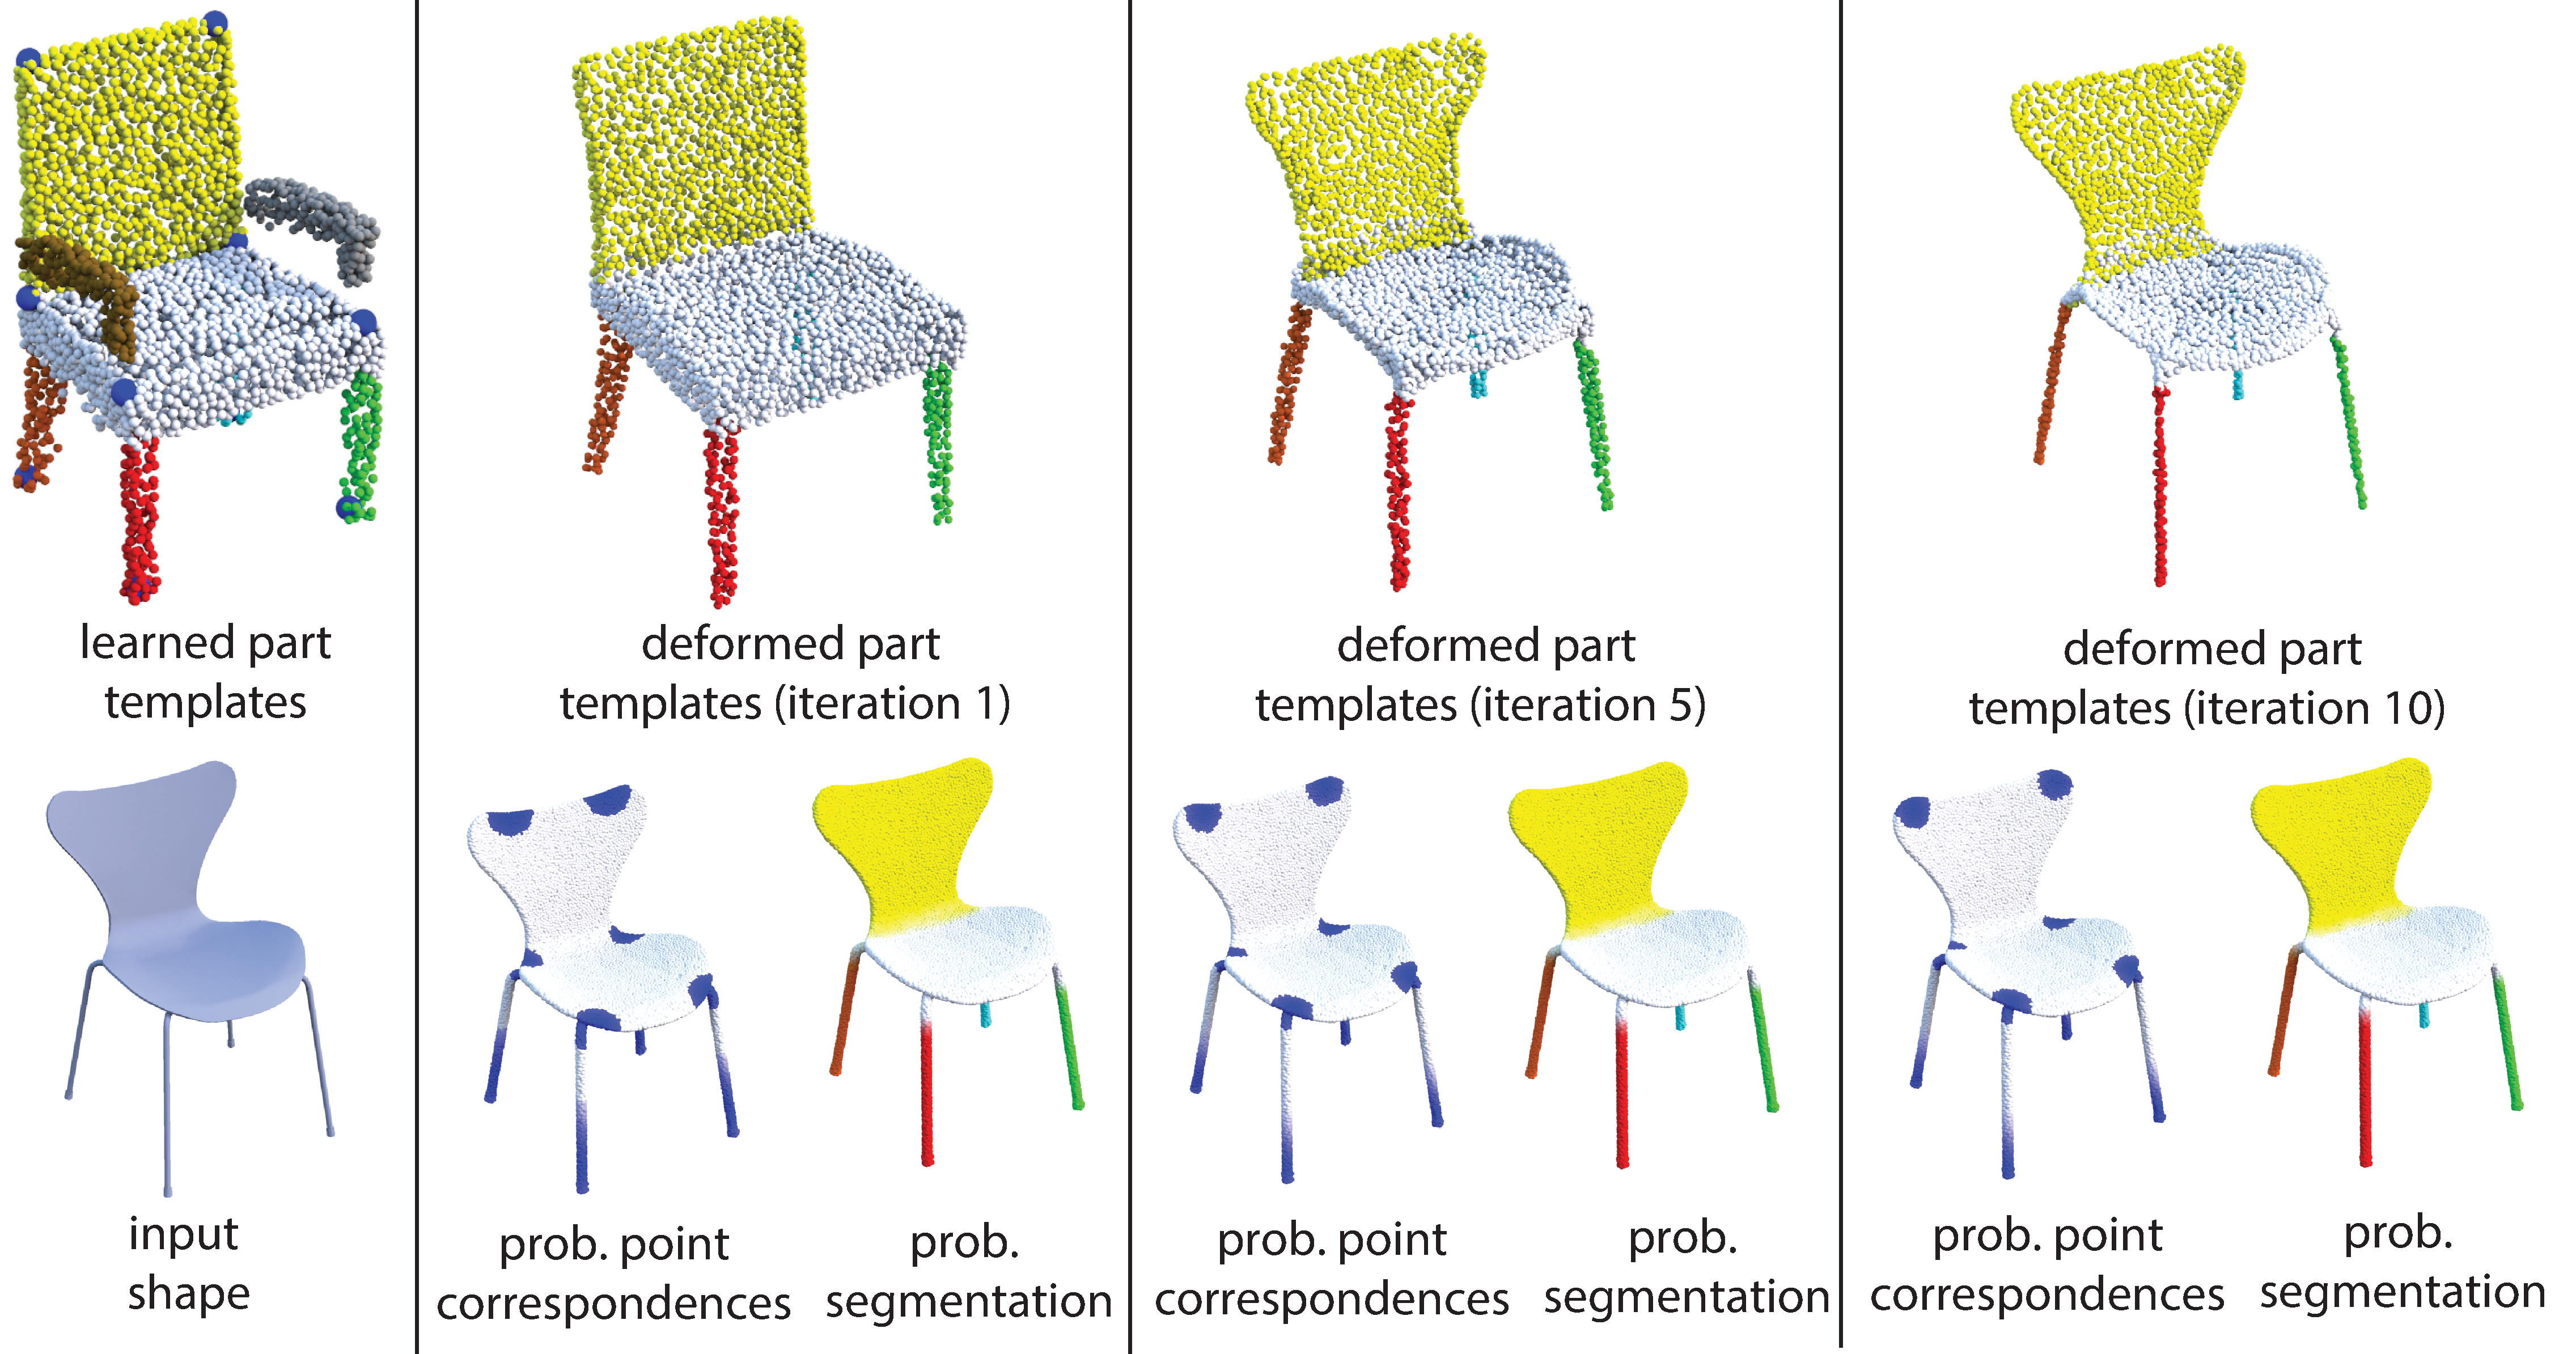
\includegraphics[width=1.02\columnwidth]{figures/deformation_iteration}
%\includegraphics[width=0.24\columnwidth]{figures/deformation_learned}
%\includegraphics[width=0.24\columnwidth]{figures/deformation_def_0}
%\includegraphics[width=0.24\columnwidth]{figures/deformation_def_1}
%\includegraphics[width=0.24\columnwidth]{figures/deformation_def_2}
%\includegraphics[width=0.24\columnwidth]{figures/deformation_target}
%\includegraphics[width=0.24\columnwidth]{figures/deformation_seg_corr_0}
%\includegraphics[width=0.24\columnwidth]{figures/deformation_seg_corr_1}
%\includegraphics[width=0.24\columnwidth]{figures/deformation_seg_corr_2}
\vskip -2mm
\caption{Given learned \rev{part templates} for four-legged chairs, our method iteratively deforms them towards an input shape through probabilistic inference. At each iteration, probability distributions over deformations, point correspondences and segmentations are inferred according to our probabilistic model (probabilistic correspondences are shown only for the points appearing as blue spheres on the learned \rev{part templates}).}
\vskip -8mm
\label{fig:deformation}
\end{figure}


Our deformation model is defined through a set of factors, each representing the degree of compatibility of different assignments to the random variables it involves. The factors control the deformation of the \rev{part templates}, the smoothness of these deformations, the fuzzy point correspondences between each \rev{part template} and input shape, and the shape segmentations. The factors are designed out of intuition and experimentation. We now explain the factors used in our model in detail. 

\textbf{Unary deformation factor.} We first define a factor that assesses the consistency of deformations of individual surface points on the \rev{part templates} with an input shape. Given an input shape $t$ represented by its sampled surface points $\bX_t$, the factor is defined as follows:
\begin{align*}
& \phi_1 (\bD_{t,k}, \bX_{t,p}, U_{t,p} = k ) = \\
& \exp\bigg\{ -.5(\bD_{t,k} - \bX_{t,p})^T \Sigma_1^{-1} (\bD_{t,k} - \bX_{t,p}) \bigg\}
\end{align*} 
where the parameter $\Sigma_1$ is a diagonal covariance matrix estimated automatically, as we explain below. The factor encourages deformations of points on the \rev{part templates} towards the input shape points that are closest to them. 

\textbf{Deformation smoothness factor.} This factor encourages smoothness in the deformations of the \rev{part templates}. Given a pair of neighboring surface points $k, k'$ on an input \rev{template}, the factor is defined as follows:
\begin{align*}
& \phi_2( \bD_{t,k}, \bD_{t,k'}, \bY_k, \bY_{k'} ) = \\
& \exp\bigg\{ -.5( (\bD_{t,k} - \bD_{t,k'})- (\bY_k - \bY_{k'}) )^T \Sigma_2^{-1} \\ 
& \,\,\,\,\,\,\,\,\,\,\,\,\,\,\,\,\,\,\,\,\,\,\,\,\,\,\,\,\,((\bD_{t,k} - \bD_{t,k'})- (\bY_k - \bY_{k'})) \bigg\}
\end{align*}
The factor favors locations of deformed points relative to their deformed neighbors that are closer to the ones on the (undeformed) \rev{part templates}. The covariance matrix $\Sigma_2$ is diagonal and is also estimated automatically. In our implementation, we use the $20$ nearest neighbors of each point $k$ to define its neighborhood. 

\textbf{Correspondence factor.} This factor evaluates the compatibility of a point on a \rev{part template} with an input surface point by comparing their geometric descriptors:
\begin{align*}
& \phi_3 ( U_{t,p} = k, \bX_t ) = \exp\bigg\{ - .5(\bff_k - \bff_{t,p})^T \Sigma_3^{-1}(\bff_k -\bff_{t,p}) \bigg\}
\end{align*}
where $\bff_k$ and $\bff_{t,p}$ are geometric descriptors evaluated on the points of the \rev{part template} and the input surface $\bX_t$ respectively, $\Sigma_3$ is a diagonal covariance matrix. Our descriptor includes geometric information from shape diameter \cite{shapira2008consistent} (under three different normalizing parameters $\alpha=1,2,4$), average geodesic distance \cite{Hilaga01}, and PCA \cite{Kim13}, forming a $10-$ dimensional vector.

\textbf{Segmentation factor.} This factor assesses the consistency of each part label with an individual surface point on an input shape. The part label depends on the fuzzy correspondences of the point with each \rev{part template}: 
\begin{align*}
\phi_4 ( S_{t,p} = l, U_{t,p} = k ) =
\begin{cases}
    1,& \text{if } label(k) = l \\
    \epsilon,& \text{if } label(k) \ne l \\
\end{cases} 
\end{align*}
where $label(k)$ represents the label of the \rev{part template} with the point $k$. The constant $\epsilon$ is used to avoid numerical instabilities during inference, and is set to $10^{-3}$ in our implementation. 
 
\textbf{Segmentation smoothness.} This factor assesses the consistency of a pair of neighboring surface points on an input shape with part labels: 
\begin{align*}
\phi_5 ( S_{t,p} = l, S_{t,p'} = l', \bX_t ) = 
\begin{cases}
    1 - \Phi_{t,p,p'},& \text{if } l \ne l' \\
    \Phi_{t,p,p'},& \text{if } l = l' \\
\end{cases} 
\end{align*}
where $p'$ is a neighboring surface point to $p$ and:
\begin{align*}
\Phi_{t,p,p'} = \exp\bigg\{ - .5(\bff_{t,p} - \bff_{t,p'})^T \Sigma_5^{-1} (\bff_{t,p} - \bff_{t,p'})  \bigg\}
\end{align*}
To define the neighborhood for each point $p$, we first segment the input shape into convex patches based on the approximate convex segmentation algorithm \cite{Asafi13}. Then we find the $20$ nearest neighbors from the patch the point $p$ belongs to. The use of information from convex patches helped our method compute smoother boundaries between different parts of the input shapes. 

\textbf{Deformation model.} Our model is defined as a Conditional Random Field (CRF) \cite{Koller09} multiplying all the above factors together and normalizing the result to express a joint probability distribution over the above random variables. 

\begin{align}
& P_{crf}( \bY, \bU, \bS, \bD | \bX ) = \frac{1}{Z(\bX)} \prod\limits_t \bigg[ \prod\limits_{k,p} \phi_1 (\bD_{t,k}, \bX_{t,p}, U_{t,p}) \nonumber \\ 
& \cdot \prod\limits_{k, k'} \phi_2( \bD_{t,k}, \bD_{t,k'}, \bY_k, \bY_{k'} ) \cdot \prod\limits_{p} \phi_3 ( U_{t,p}, \bX_t ) \nonumber  \\
& \cdot \prod\limits_{p} \phi_4 ( S_{t,p}, U_{t,p} ) \cdot \prod\limits_{p, p'} \phi_5 ( S_{t,p}, S_{t,p'}, \bX_t ) \bigg]
\label{eq:objective}
\end{align}

\textbf{Mean-field inference.} Using the above model, our method infers probability distributions for \rev{part templates} and deformations, as well as shape segmentations and correspondences. To perform inference, we rely on the mean-field approximation theory due to its efficiency and guaranteed convergence properties. We approximate the original probability distribution $P_{crf}$ with another simpler distribution $Q$ such that the KL-divergence between these two distributions is minimized: 
\begin{align*}
P_{crf}( \bY, \bU, \bS, \bD | \bX )  \approx Q( \bY, \bU, \bS, \bD | \bX )
\end{align*}
where the approximating distribution $Q$ is a product of individual distributions associated with each variable:
\begin{align*}
& Q( \bY, \bU, \bS, \bD | \bX ) = \\
& \prod\limits_k Q( \bY_k ) \prod\limits_{t,k} Q( \bD_{t,k} ) \prod\limits_{t,p} Q( U_{t,p} ) \prod\limits_{t,p} Q( S_{t,p} )
\end{align*}

For continuous variables, we use Gaussians as approximating individual distributions, while for discrete variables, we use categorical distributions. We provide all the mean-field update derivations for each of the variables in the supplementary material. Learning the \rev{part templates} entails computing the expectations of \rev{part template} variables $\bY_k$ with respect to their approximating distribution $Q(\bY_k)$. For each \rev{part template} point $\bY_k$, the mean-field update is given by:

\begin{align*}
& Q(\bY_k) \propto \exp\bigg\{ -.5(\bY_k - \bmu_k )^T \Sigma_2^{-1} ( \bY_k -  \bmu_k )  \bigg\}
\end{align*}
where:
\begin{align*}
\bmu_k = \frac{1}{|\mN(k)|} \sum\limits_{k'} \big( \Ex_Q[\bY_{k'}] + \frac{1}{T}\sum\limits_t(\Ex_Q[\bD_{t,k}] - \Ex_Q[\bD_{t,k'}]) \big)
\end{align*}
and $\mN(k)$ includes all neighboring points $k'$ of point $k$ on the \rev{part template}. As seen in the above equation, to compute the mean-field updates, we need to compute expectations over deformations of \rev{part templates}. However, to compute these expectations, we require an initialization for the \rev{part templates}, as described next. 

\textbf{Clustering.} The first step of our method is to cluster the input shapes into groups of structurally similar shapes. For this purpose, we define a dissimilarity measure between two shapes based on our unary deformation factor. We measure the amount of deformation required to map the points of one shape towards the corresponding points of the other shape in terms of their Euclidean distance, and vice versa. 
%To compute the closest corresponding point for a query point, we only consider points whose normal has the same direction with the normal of the query point. 
For small datasets (with less than 100 shapes), we compute the dissimilarities between all-pairs of shapes, then use the affinity propagation clustering algorithm \cite{Frey07}. The affinity propagation algorithm takes as input dissimilarities between all pairs of shapes, and outputs a set of clusters together with a set of representative, or exemplar, shape per cluster. We note that another possibility would be to use all the factors of the model to define a dissimilarity measure, however, this proved to be computationally too expensive. For larger datasets, we compute a graph over the input shapes, where each node represents a shape, and edges connect shapes which are similar according to a shape descriptor \cite{Kim12}. We compute distances for pairs of shapes connected with an edge, then embed the shapes with the Isomap technique \cite{Tenenbaum:2000:GGF} in a $20$-dimensional space. We use the distances in the embedded space as dissimilarity metric for affinity propagation. 

As mentioned above, affinity propagation also identifies a representative, or exemplar, shape per cluster. In the case of manual initialization of our method, we ask the user to segment each identified exemplar shape per group, or let him select a different exemplar shape if desired. In the case of non-manual segmentation initialization, we rely on a co-segmentation technique to get an initial segmentation of each exemplar shape. In our implementation we use the co-segmentation results provided by Kim et al. \shortcite{Kim13}. Even if the initial segmentation of the exemplar shapes is approximate, our method updates and improves the segmentations for all shapes in the collection based on our probabilistic deformation model, as demonstrated in the results. To ensure that the identified exemplar shape has all (or most) representative parts per cluster in the case of automatic initialization, we modify the clustering algorithm to force it to select an exemplar from the shapes with the largest number of parts per cluster based on the initial shape co-segmentations. Figure \ref{fig:hierarchy} shows the detected clusters for a small chair dataset and user-specified shape segmentations for each exemplar shape per cluster. 

\textbf{Inference procedure and parameter learning.} Given the clusters and initially provided parts for exemplar shapes, the mean-field procedure follows the Algorithm \ref{algorithm}. At line 1, we initialize the approximating distributions for the \rev{part templates} according to a Gaussian centered at the position of the surface points on the provided exemplar parts. We then initialize the deformed versions of the \rev{part templates} using the provided exemplar parts after aligning them with each exemplar shape (lines 2-5). Alignment is done by finding the least-squares affine transformation that maps the exemplar shapes with the shapes of their group. The affine transformation is used to account for anisotropic scale differences between shapes in each group. We initialize the approximating distributions for correspondences and segmentations with uniform distributions (lines 6-9). Then we start an outer loop (line 10) during which we update the covariance matrices (line 11) and execute an inner loop for updating the approximating distributions for segmentations, correspondences and deformations for each input shape (lines 12-24). The covariance matrices are computed through piecewise training \cite{Sutton05} on each factor separately using maximum likelihood. We provide the parameter updates in the supplementary material. Finally, we update the distributions on \rev{part templates} (line 25). The outer loop for updating the \rev{part templates} and parameters requires $5-10$ iterations to reach convergence in our datasets. Convergence is checked based on how much the inferred point position on the \rev{part template} deviate on average from the ones of the previous iteration.  For the inner loop, we practically found that running more mean-field iterations ($10$ in our experiments) for updating the deformations helps the algorithm converge to better segmentations and correspondences. During the inference procedure, our method can infer negligible probability (below $10^{-3}$) for one or more part labels for all points on an input shape. This happens when an input shape has parts that are subset of the ones existing in its group. In this case, the \rev{part templates} missing from that shape are deactivated e.g., Figure \ref{fig:deformation} demonstrates this case where the input shape does not have armrests. 

\textbf{High-level part template learning.} Learning the \rev{part templates} at the top level of hierarchy follows the same algorithm as above with different input. Instead of the shapes in the collection, the algorithm here takes as input the learned \rev{part templates} per group. For initialization, we try each part from the lower level to initialize each higher-level \rev{part template} per label, and select the one with highest probability according to our model (Equation \ref{eq:objective}). The \rev{part templates}, deformations and correspondences are updated according to Algorithm \ref{algorithm}. For this step, we omit the updates for segmentations, since the algorithm works with individual parts. We note that it is straightforward to extend our method to handle more hierarchy levels of \rev{part templates} (e.g., splitting the clusters into sub-clusters also leading to the use of more exemplars per shape type, or group) by applying the same algorithm hierarchically and using a hierarchical version of affinity propagation \cite{Givoni11}. Experimentally, we did not see any significant benefit from using multiple exemplars per group at least in the datasets we used.



\begin{algorithm}
\LinesNumbered
\SetNlSty{texttt}{}{:}
\SetKwInOut{Input}{input}\SetKwInOut{Output}{output}
\Input{Input collection and initially segmented parts of exemplar shapes}
\Output{Learned \rev{part templates}, shape correspondences and segmentations}
\BlankLine

Initialize $\Ex_Q[\bY_k]$ from the position of the exemplar shape part points\;

\For{\textnormal{each shape} $t\leftarrow 1$ \KwTo $T$}
 {
  \For{\textnormal{each part template point} $k\leftarrow 1$ \KwTo $K$}
  {   
   Initialize $\Ex_Q[\bD_{t,k}]$ from the aligned part templates with the shape $t$\;
  }
  \For{\textnormal{each surface point} $p\leftarrow 1$ \KwTo $P$}
  {     
   Initialize $Q(U_{t,p})$ and $Q(S_{t,p})$ to uniform distributions\;
  }
 }
 
\Repeat{convergence}
{
  Update covariance matrices $\bSigma_1, \bSigma_2, \bSigma_3, \bSigma_5$;
        
  \Repeat{convergence}
  {     
        \For{\textnormal{each shape} $t\leftarrow 1$ \KwTo $T$}
         {  
            \For{\textnormal{each surface point} $p\leftarrow 1$ \KwTo $P$}
            { 
                  update correspondences $Q(\bU_{t,p})$\;
                  update segmentations $Q(\bS_{t,p})$\;
            }  
            \For{iteration $\leftarrow 1$ \KwTo $10$}
            { 
              \For{\textnormal{each part template point} $k\leftarrow 1$ \KwTo $K$}
                { 
                     update deformations $Q(\bD_{t,k})$;
                }
            }
         }
  }
  update part templates $Q(\bY)$\;
}
\vskip 1mm
\caption{Mean-field inference procedure.}
\label{algorithm}
\end{algorithm}




